\lesson{Origins of Quantum Theory}
\begin{bulleted-list}
    \item \textbf{Max Planck} is credited with starting the quantum revolution with a surprising interpretation
        of the experimental results obtained from the study of the light emitted by hot objects
    \item \textbf{Gustav Kirchhoff} was interested in the light emitted by blackbodies
    \item The term \textbf{blackbody} is used to describe an ideal, perfectly black object that
        does not reflect any light and emits various different forms of light (electromagnetic
        radiation) as a result of its temperature
\end{bulleted-list}

\subsection{Planck's Quantum Hypothesis}
\begin{bulleted-list}
    \item As a solid is heated, it changes colours. Initially it is red, then white. Recall
        that white is a combination of all colours, so the light emitted by the hotter
        object must now be accompanied by, for example, blue light
    \item The changes in the colours and the corresponding spectra do not depend on the composition
        of the solid
    \item The intensity (brightness) of the different colours observed in the spectrum of emitted
        light resembles a bell curve. See Figure \ref{fig:intensity-wavelength-graph}
\end{bulleted-list}

\begin{figure}[ht!]
    \centering
    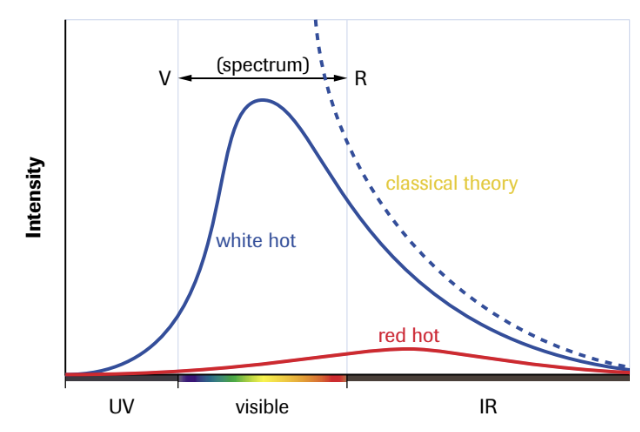
\includegraphics[width=0.7 \textwidth]{../figures/intensity-wavelength-graph.png}
    \caption{The solid lines show the intensity of the colours of light emitted by a red-hot
        wire and a white-hot wire. Notice how the curve becomes higher and shifts toward the
        higher UV as the temperature increases. The dotted line represents the predicted curve
        for a white-hot object, according to the classical theory before Planck}
    \label{fig:intensity-wavelength-graph}
\end{figure}

\begin{bulleted-list}
    \item For many years, scientists struggled to explain the curves shown in Figure \ref{fig:intensity-wavelength-graph}.
        Some were able to describe it at the endpoints, but not the overall curve obtained from
        experiments. See Figure \ref{fig:classical-theory-intensity-energy-graph}
    \item Planck hypothesized that the energies of the oscillating atoms in the heated solid were
        multiples of a small quantity of energy; in other words, energy is \textbf{not continuous}
    \item Einstein later pointed out that the inevitable conclusion of Planck's hypothesis is that
        light emitted by a hot solid is also quantized--it comes in ``bursts'', not as a
        continuous stream of energy
    \item One little burst or packet of energy is called \textbf{quantum} of energy
\end{bulleted-list}

\begin{figure}[ht!]
    \centering
    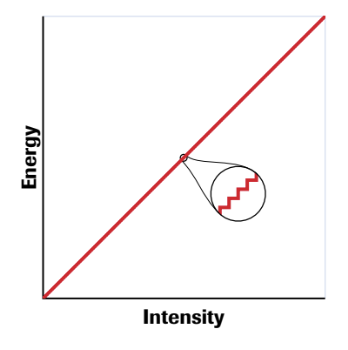
\includegraphics[width=0.5 \textwidth]{../figures/classical-theory-intensity-energy-graph.png}
    \caption{For many years, scientists could not explain the intensity curve, because they
        believed that as the intensity of light changes, the total energy increases continuously.
        However, as a consequence of Planck's work, Einstein suggested the slope is actually
        a staircase with tiny steps, where each step is a quantum of energy}
    \label{fig:classical-theory-intensity-energy-graph}
\end{figure}

\begin{bulleted-list}
    \item An interpretation of the evidence from heating a solid is that a sequence of quanta
        emissions from IR to red to blue to UV occurs. A logical interpretation is that as the
        temperature increased, the proportions of each larger quantum becomes greater
    \item The temperature of a heated object is due to a complex combination of the number and
        kind of quanta
\end{bulleted-list}

\begin{sample}{How would observations of a star allow astronomers to obtain the temperature of
    the star?}
    The colour of the star corresponds to its temperature. It is important to account for luminosity
    instead of apparent colour because the intensities are different at different distances
\end{sample}

\begin{sample}{Liquids and solids, when heated, produce continuous spectra. What kind of spectrum
    is produced by a heated gas?}
    Heated gas produces a line spectrum. This is because the quantized energy causes the transition
    of electrons between energy levels, releasing energy, which produces a line spectrum.
\end{sample}

\subsection{The Photoelectric Effect}
\begin{bulleted-list}
    \item Early on, scientists believed that light acted like a stream of particles, or a wave
        so to speak. Many scientists, including Newton, bitterly opposed this. But, evidence from
        experiments with, for example, reflection, refraction, and diffraction facourde the
        wave hypothesis over the particle view
    \item In the mid-19th century, \textbf{James Maxwell} proposed a theory explaining the known
        properties of light, electricity, and magnetism. He proposed that light is an electromagnetic
        wave composed of electric and magnetic fields that can exert forces on charged particles. This
        electromagnetic-wave theory, known as the \textbf{classical theory of light} became widely
        accepted
    \item The spectrum derived from this theory is seen in Figure \ref{fig:maxwell-electronagmetic-spectrum}
    \item The reason why light is sometimes a wave and other times a particle is because scientists
        used the \textbf{black-box model}. We cannot say for sure because we are only observing
        the inputs and outputs, thus we treat light as both a wave and particle
\end{bulleted-list}

\begin{figure}[ht!]
    \centering
    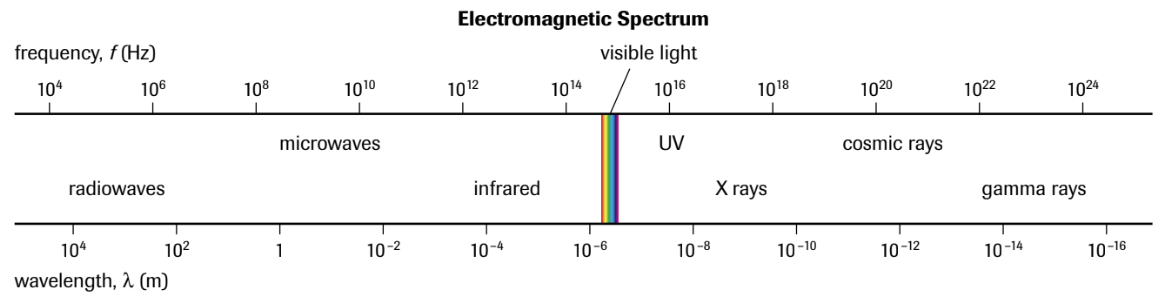
\includegraphics[width=\textwidth]{../figures/maxwell-electromagnetic-spectrum.png}
    \caption{The electromagnetic spectrum originally prediced by Maxwell. It includes all forms
        of electromagnetic radiation from very short wavelength gamma ($\gamma$) rays to oridnary
        visible light to very long wavelength radio waves}
    \label{fig:maxwell-electronagmetic-spectrum}
\end{figure}

\begin{bulleted-list}
    \item \textbf{Heinrich Hertz} discovered the \textbf{photoelectric effect} by accident in 1887. It
        involves the effect of electromagnetic radiation or light on substances, particularly 
        certain metals. See Figure \ref{fig:photoelectric-effect}
    \item According to the classical theory, the intensity/brightness of the light shone on
        the metal would determine the kinetic energy of the liberated electrons; the brighter
        the light, the greater the current. But this was shown to be \textbf{false}
    \item Further experimental work showed that the frequency (colour/energy) of the light was
        the most important characteristic of the light in generating current. In other words,
        the classical theory was unacceptable for explaining the photoelectric effect
    \item Einstein built on Planck's idea of a quantum of energy to propose that light consisted
        of a stream of energy packets or quanta--later called \textbf{photons}. A photon of red 
        light contains less energy than a photon of UV light, for example.
    \item Einstein suggested that the ejection of an electron from the metal surface could be 
        explained in terms of \textbf{photon-electron} collision. The energy of the photon
        is transferred to the electron, some of the energy used for the electron to break free
        from the atom and the rest is left over as kinetic energy of the ejected atom
    \item The key thing is that the electron cannot break free from the atom unless a cretain
        minimum quantity of energy is absorbed from a single photon
\end{bulleted-list}

\begin{figure}[ht!]
    \centering
    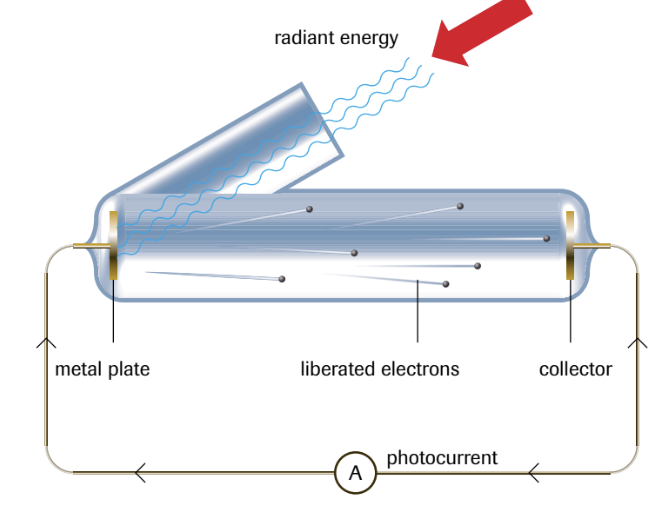
\includegraphics[width=\textwidth]{../figures/photoelectric-effect.png}
    \caption{In the photoelectric effect, light shining on a metal plate liberates electrons from
        the metal surface. The ammeter (A) records the electric current in the circuit. In other
        words, light shining on a metal plate magically produced current}
    \label{fig:photoelectric-effect}
\end{figure}
